\documentclass[11pt]{report}
\usepackage[utf8]{inputenc}
\usepackage[T1]{fontenc}
\usepackage[french]{babel}
\usepackage{geometry}
\usepackage{tikz} 
\usepackage{amsmath}
\usepackage{amssymb}
\usepackage{ifthen}
\usepackage{fancybox}
\usepackage{fancyhdr}
\geometry{left=1cm , right=1cm , top=1.5 cm , bottom=1.5cm}
\usepackage{color}
\usepackage{soul}
\usepackage{graphicx}
\thispagestyle{empty}
\usepackage[utf8]{inputenc}
\usepackage[T1]{fontenc}
\usepackage{fullpage}
\usepackage{caption}
\usepackage{subcaption}
\usepackage{lipsum}


\begin{document}
Dans cette section nous allons effectuer des tests sur les différentes méthodes de détection des points aberrants,où chaque méthode possède un paramètre estimé manuellement ,alors notre but  c'est de faire varier ce paramètre dans chaque méthode et regarder si avec une faible variation d'un paramètre le résultat change faiblement ou s'il change complètement

\subsection*{Méthode inter-quartiles}
Dans un premier temps on a fixé le paramètre  coeff de cette méthode à $coeff=0.5$ et c'est le paramétré estimé manuellement \\
si on essaye de diminuer la valeur de notre paramètre coeff à chaque fois on remarque que  notre algorithme détecte plus de points aberrants qu'au début  et même il considère des ponits aberrants sur notre spline ce qu'est n'est pas logique \\
et si on essaye d'augmenter aussi notre paramètre à chaque fois on va remarquer que notre méthode va détecter moins de points aberrants jusqu'à son absence à la valeur 3.1 \\\vspace{2cm}

\begin{figure}[!htb]
\minipage{0.4\textwidth}
  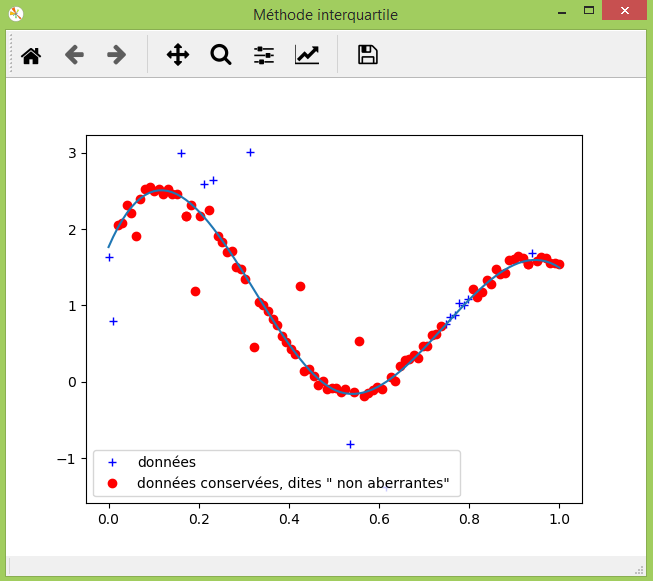
\includegraphics[width=\linewidth]{quan.png}
  \caption{coeff=0.5}\label{fig:awesome_image1}
\endminipage\hfill
\minipage{0.4\textwidth}
  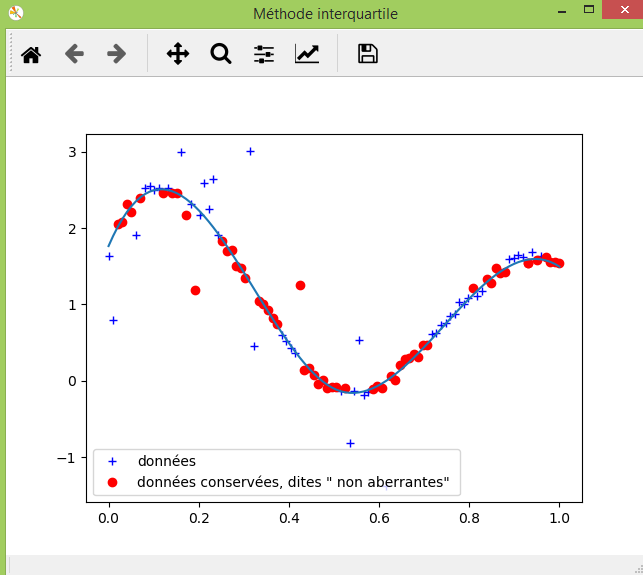
\includegraphics[width=\linewidth]{quam.png}
  \caption{coeff=0.05}\label{fig:awesome_image2}
\endminipage\hfill
\end{figure}

\begin{figure}[!htb]
\minipage{0.4\textwidth}%
  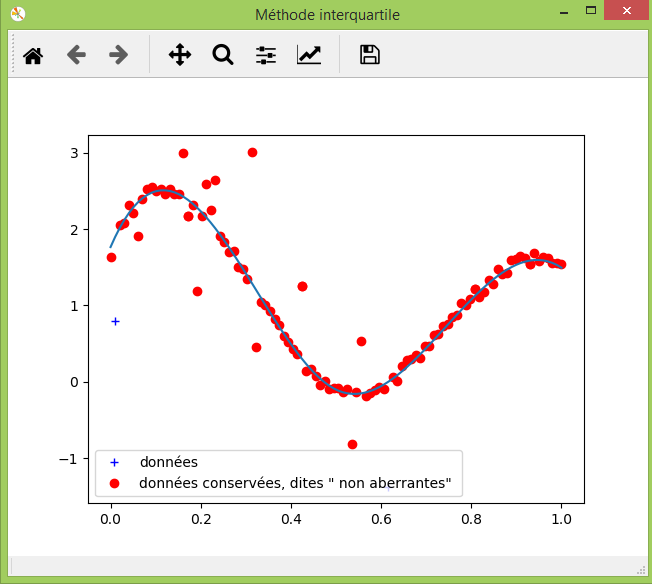
\includegraphics[width=\linewidth]{quap.png}
  \caption{coeff=1.4}\label{fig:awesome_image3}
\endminipage
\minipage{0.4\textwidth}%
  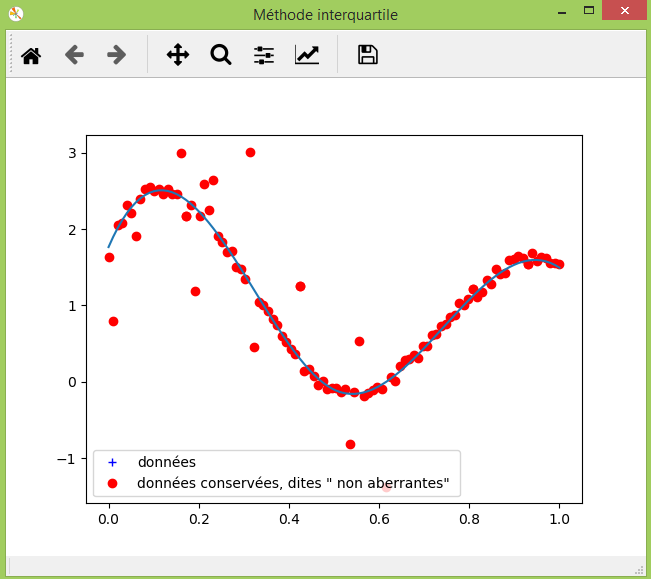
\includegraphics[width=\linewidth]{quas.png}
  \caption{coeff=3.1}\label{fig:awesome_image3}
\endminipage
\end{figure}


 
\newpage
\subsection*{Méthode de chauvenet}
c'est presque le même principe avec la méthode précédente juste ici une augmentation du paramètre tau de la méthode va  détecter plus de points aberrants qu'au début et  si on essaye de diminuer  aussi notre paramètre à chaque fois on va remarquer que notre méthode va détecter moins de points aberrants. \\ et voici les testes de cette méthode avec différentes valeur du paramètre tau: 
 \begin{figure}[!htb] %on ouvre l'environnement figure
 
\minipage{0.32\textwidth}% 
\includegraphics[width=\linewidth]{chauvn.PNG} %ou image.png, .jpeg etc.

\caption{tau=0.5} %la légende
\label{coeff_05qua} %l'étiquette pour faire référence à cette image
\endminipage
\minipage{0.32\textwidth}%
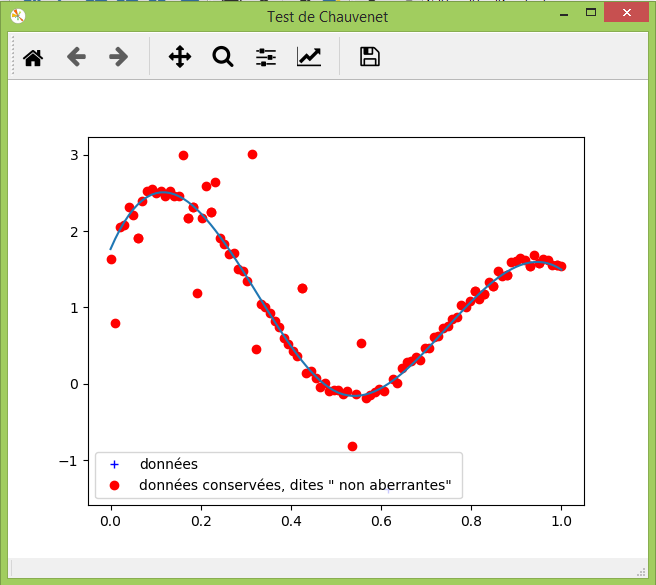
\includegraphics[width=\linewidth]{chauvm.PNG}  
\caption{tau=0.05}
\label{coeff_005qua}
\endminipage
\minipage{0.32\textwidth}%
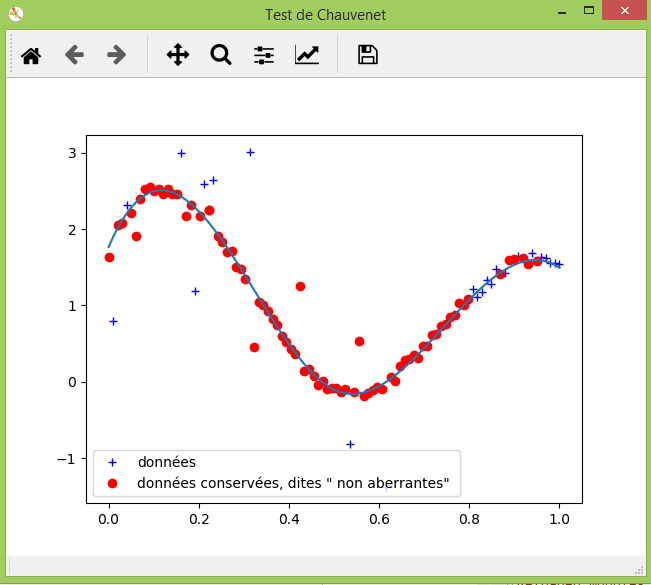
\includegraphics[width=\linewidth]{chauvp.PNG}  
\caption{tau=1.4}
\label{coeff_1.4qua}

\endminipage

\end{figure} 
 \subsection*{Remarque:}
 c'est le même cas dans toutes les méthodes qui reste du coup on a  donné des testes sur chaque méthode avec des différents paramètres 
 \subsection*{Méthode de thompson}
 



  \begin{figure}[!htb] %on ouvre l'environnement figure
  \minipage{0.32\textwidth}%
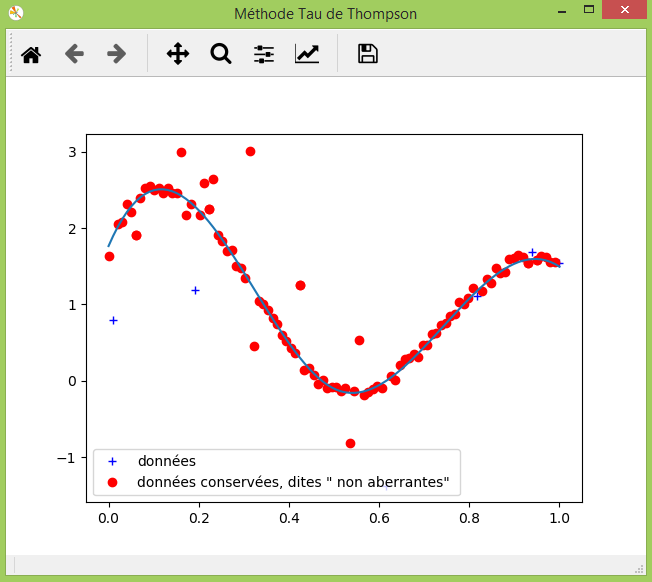
\includegraphics[width=\linewidth]{thomn.PNG} %ou image.png, .jpeg etc.
\caption{alpha=1.995} %la légende
\label{alpha1995} %l'étiquette pour faire référence à cette image
\endminipage
\minipage{0.32\textwidth}%
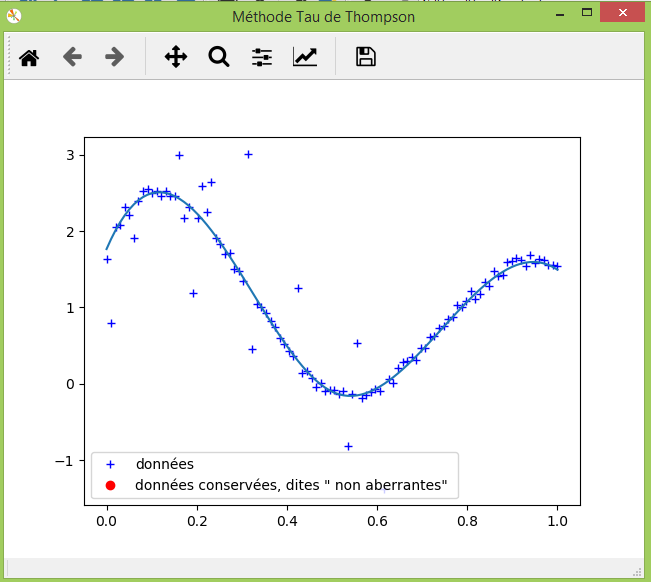
\includegraphics[width=\linewidth]{thomm.PNG}  
\caption{alpha=0.995}
\label{alpha_0995}
\endminipage
\minipage{0.32\textwidth}%
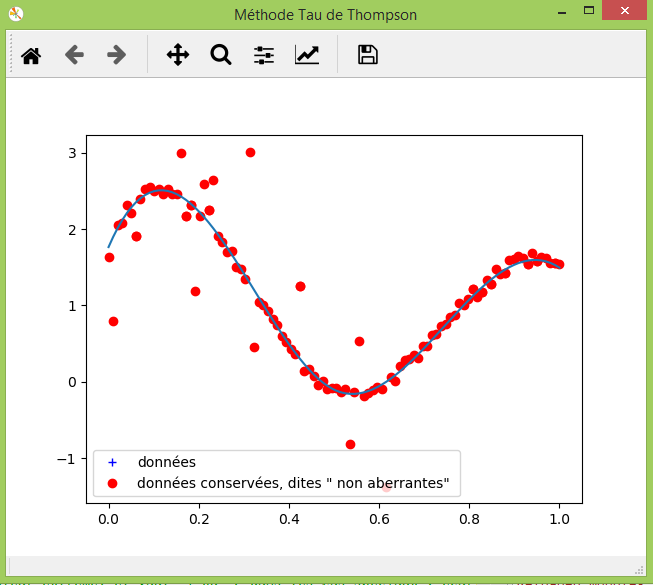
\includegraphics[width=\linewidth]{thoms.PNG}  
\caption{alpha=2.995}
\label{alpha_2995}
\endminipage



\end{figure}

\newpage
\subsection*{Méthode de grubbs}
 
 \begin{figure}[!htb] %on ouvre l'environnement figure
  \minipage{0.32\textwidth}%
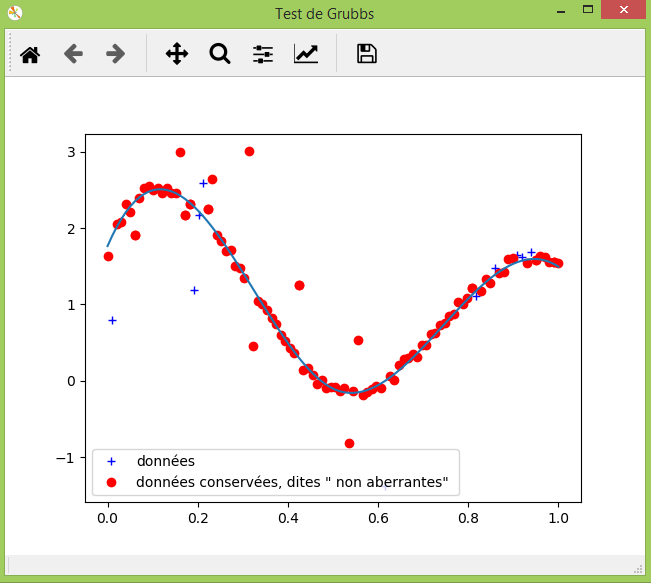
\includegraphics[width=\linewidth]{grun.PNG} %ou image.png, .jpeg etc.
\caption{alpha=5/100} %la légende
\label{alpha1995} %l'étiquette pour faire référence à cette image
\endminipage
\minipage{0.32\textwidth}%
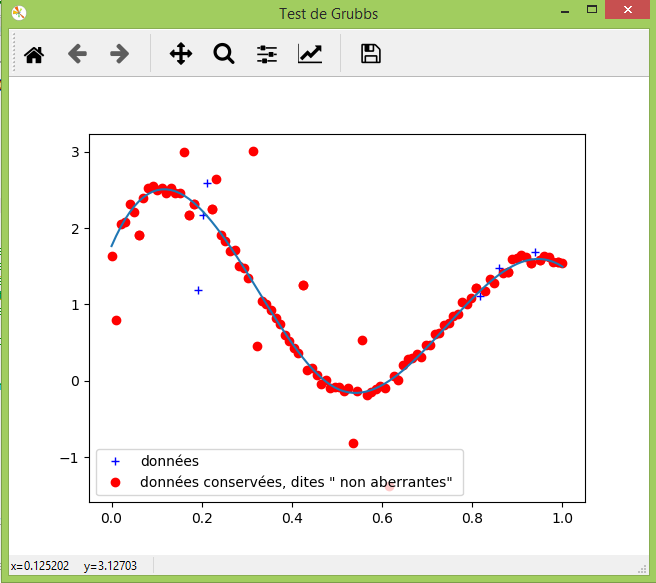
\includegraphics[width=\linewidth]{gru005.PNG}  
\caption{alpha=0.5/100}
\label{alpha_0995}
\endminipage
\minipage{0.32\textwidth}%
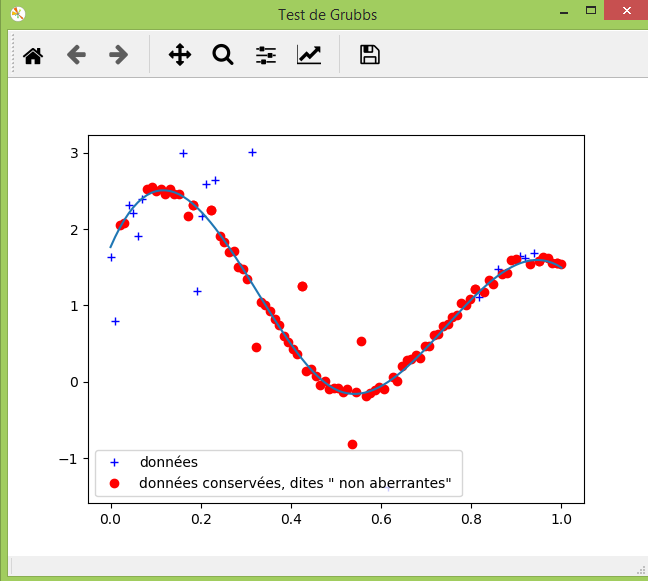
\includegraphics[width=\linewidth]{gru50.PNG}  
\caption{alpha=50/100}
\label{alpha_2995}
\endminipage



\end{figure}

\subsection*{methode de deviation extreme student}
 \begin{figure}[!htb] %on ouvre l'environnement figure
  \minipage{0.32\textwidth}%
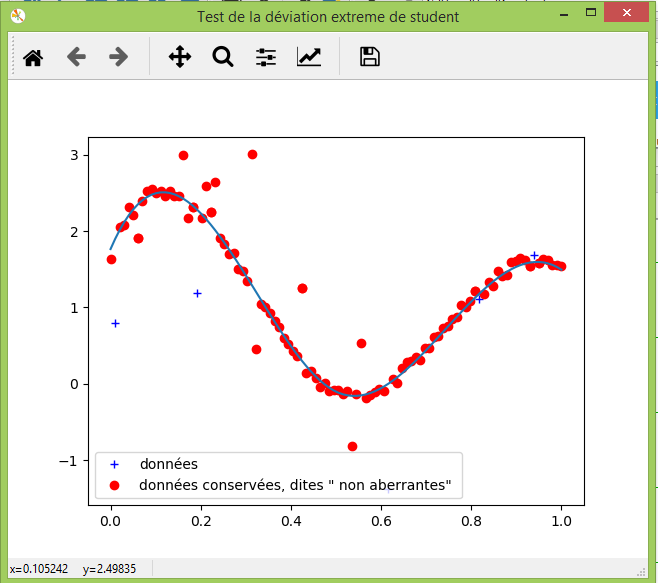
\includegraphics[width=\linewidth]{extn.PNG} %ou image.png, .jpeg etc.
\caption{alpha=5/100} %la légende
\label{alpha1995} %l'étiquette pour faire référence à cette image
\endminipage
\minipage{0.32\textwidth}%
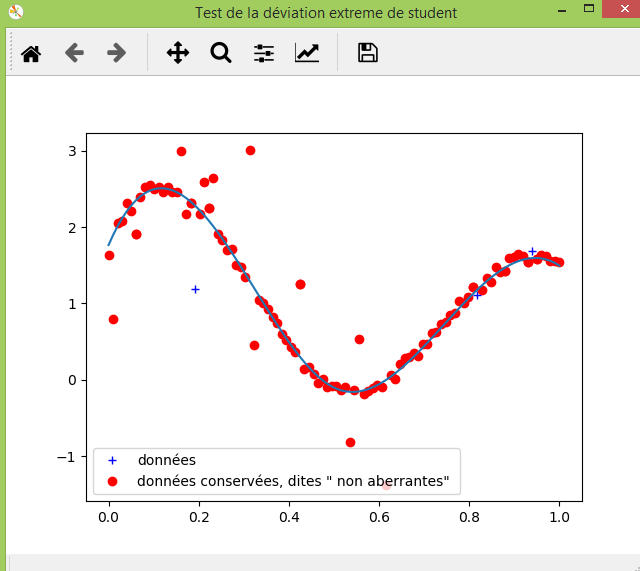
\includegraphics[width=\linewidth]{ext005.PNG}  
\caption{alpha=0.5/100}
\label{alpha_0995}
\endminipage
\minipage{0.32\textwidth}%
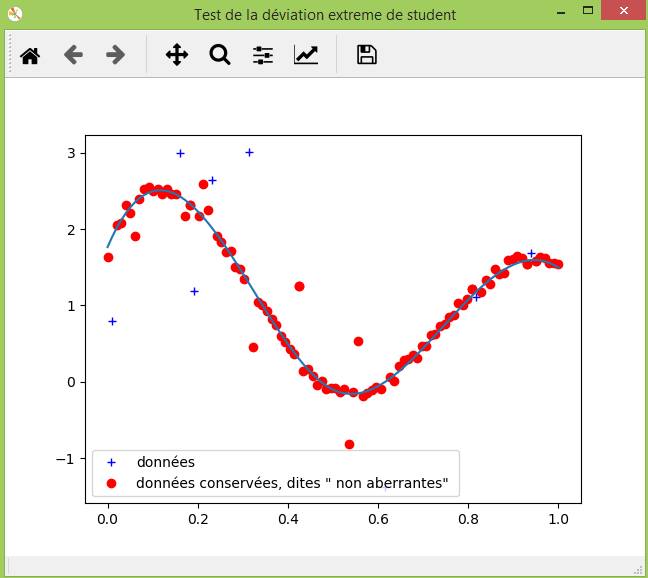
\includegraphics[width=\linewidth]{ext50.PNG}  
\caption{alpha=50/100}
\label{alpha_2995}
\endminipage
\end{figure}

\newpage
\subsection*{methode de KMN}
 \begin{figure}[!htb] %on ouvre l'environnement figure
  \minipage{0.32\textwidth}%
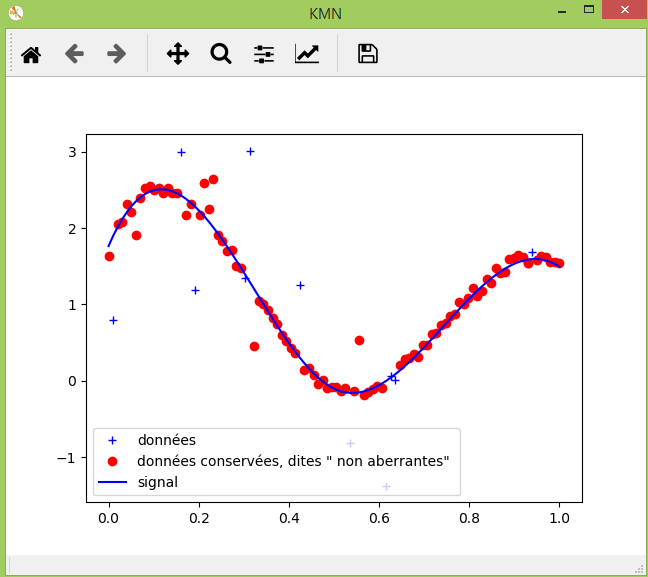
\includegraphics[width=\linewidth]{kmnn.PNG} %ou image.png, .jpeg etc.
\caption{paramètre =15} %la légende
\label{m15} %l'étiquette pour faire référence à cette image
\endminipage
\minipage{0.32\textwidth}%
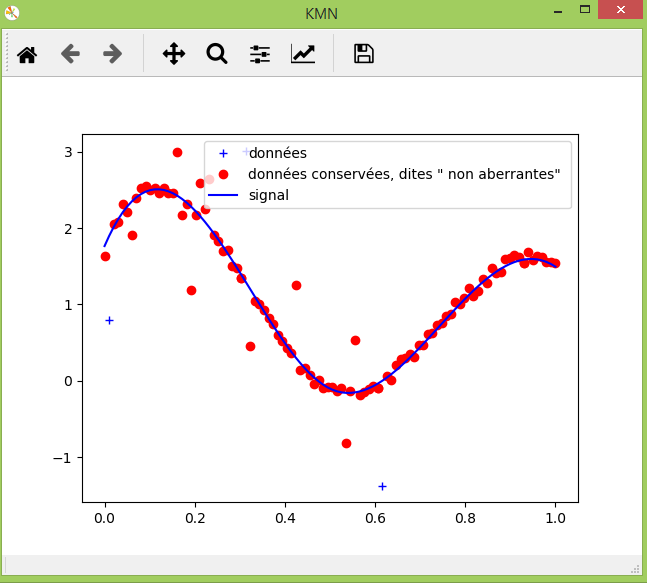
\includegraphics[width=\linewidth]{kmn5.PNG}  
\caption{paramètre=5}
\label{m5}
\endminipage
\minipage{0.32\textwidth}%
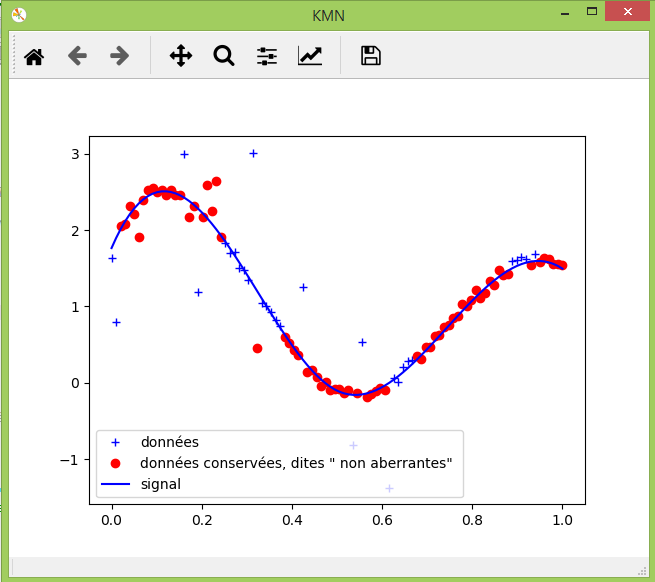
\includegraphics[width=\linewidth]{kmn35.PNG}  
\caption{paramètre=35}
\label{m35}
\endminipage

\end{figure}

\subparagraph{Remarque 1:} ces testes nous ont permis de choisir (Estimations manuelle) le paramètre idéal pour  chaque méthode 
\subparagraph{Remarque 2:} on a effectuer les testes même dans le cas non stationnaire pour chaque méthode et le changement à chaque fois suit la même logique que dans le cas stationnaire \vspace{3cm}

\subparagraph{exemple:}méthode de chevenent dans le cas non stationnaire:
\begin{figure}[!htb] %on ouvre l'environnement figure
 
\minipage{0.32\textwidth}% 
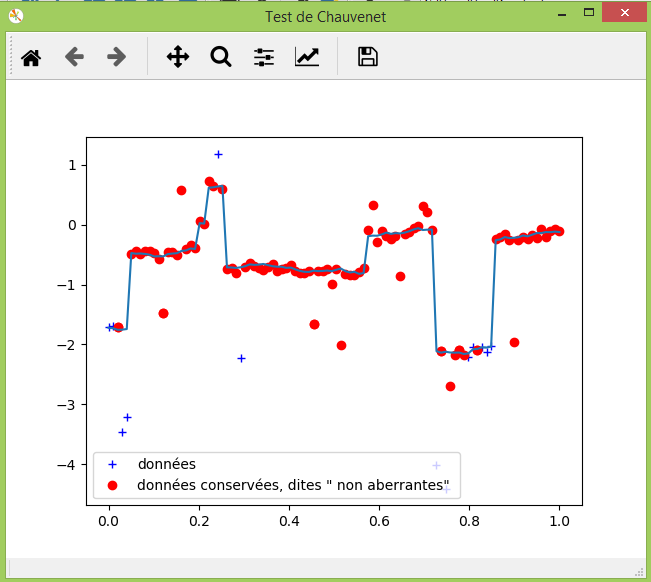
\includegraphics[width=\linewidth]{nst05.PNG} %ou image.png, .jpeg etc.

\caption{tau=0.5} %la légende
\label{coeff_05qua} %l'étiquette pour faire référence à cette image
\endminipage
\minipage{0.32\textwidth}%
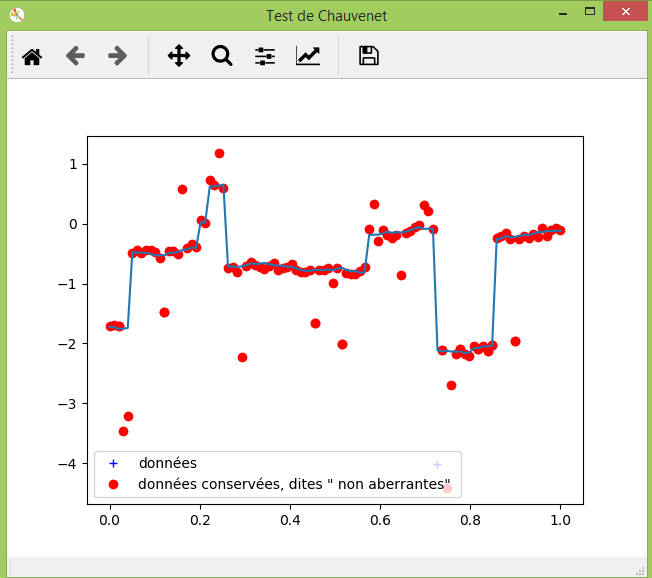
\includegraphics[width=\linewidth]{nst005.PNG}  
\caption{tau=0.005}
\label{coeff_005qua}
\endminipage
\minipage{0.32\textwidth}%
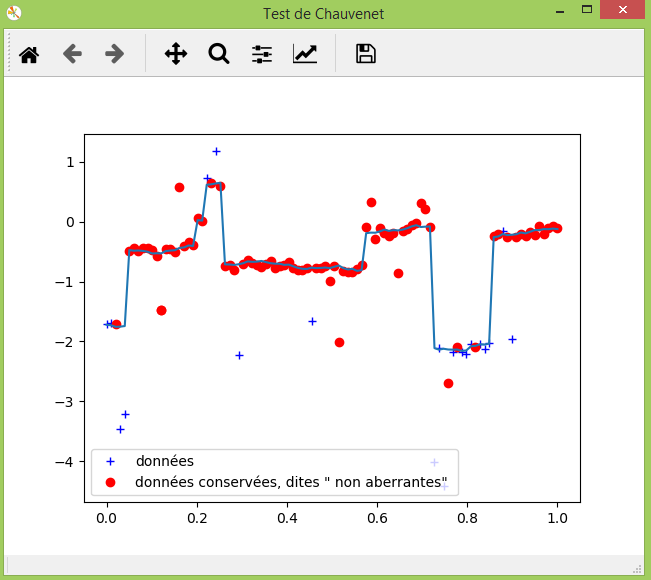
\includegraphics[width=\linewidth]{nst14.PNG}  
\caption{tau=1.4}
\label{coeff_1.4qua}

\endminipage

\end{figure} 
\end{document}
